\documentclass{beamer}
\usepackage{float}
\usepackage{graphicx}
\usepackage{marginnote}
\usepackage{pgfgantt}
\usepackage{pdflscape}
\usepackage{wrapfig}
\usepackage{tikz}

\usepackage{listings}
\usepackage{color}
\usepackage{pgfplots}
\usepackage{filecontents}
\pgfdeclarelayer{background}
\pgfdeclarelayer{foreground}
\pgfsetlayers{background,main,foreground}

\usetikzlibrary{matrix}
\usetikzlibrary{shapes,arrows}
\renewcommand{\footnoterule}{%
  \kern -3pt
  \hrule width \textwidth height 0.5pt
  \kern 2pt
}
\tikzstyle{decision} = [diamond, draw, fill=white!20, 
    text width=6em, text badly centered, node distance=3cm, inner sep=1pt]
\tikzstyle{block} = [rectangle, draw, fill=white!20, 
    text width=5em, text centered, rounded corners, minimum height=3em]
\tikzstyle{line} = [draw, -latex']
\tikzset{
  treenode/.style = {align=center, inner sep=0pt, text centered,
    font=\sffamily},
 arn_n/.style = {treenode, circle, white,  font=\sffamily, draw=black,
    fill=black, text width=1.5em}
}
\tikzset{
    maxfitnessorgen /.style={
        /pgfplots/execute at end plot visualization={\draw [current plot style, dashed] (@auxnode.center) -- ($(@auxnode.center)!10cm!(@auxnode.east)$);}
    },
    maxfitnessorgen nodestyle/.style={
        pos=1, inner sep=0pt, sloped, alias=@auxnode
    }
}
\mode<presentation> {

\setbeamertemplate{footline}[page number] % To replace the footer line in all slides with a simple slide count uncomment this line

\setbeamertemplate{navigation symbols}{} % To remove the navigation symbols from the bottom of all slides uncomment this line
}

\usepackage{graphicx} % Allows including images
\usepackage{booktabs} % Allows the use of \toprule, \midrule and \bottomrule in tables
\usepackage{xcolor}
\title[Short title]{Random Number Generation using Genetic Programming: Demonstration} % The short title appears at the bottom of every slide, the full title is only on the title page

\author{Philip Leonard} % Your name
\institute[UoL] % Your institution as it will appear on the bottom of every slide, may be shorthand to save space
{
University of Liverpool \\ % Your institution for the title page
\medskip
Primary Supervisor: Dr. David Jackson\\ Secondary Supervisor: Professor Paul E. Dunne\\
\medskip
\textit{sgpleona@student.liverpool.ac.uk} % Your email address
}
\date{} % Date, can be changed to a custom date

\definecolor{lblue}{HTML}{33B5E5}
\definecolor{lgrey}{HTML}{7F8C8D}
\definecolor{lpurple}{HTML}{AA66CC}
\definecolor{lgreen}{HTML}{99CC00}
\definecolor{lorange}{HTML}{FFBB33}
\definecolor{lred}{HTML}{FF4444}
\definecolor{dblue}{HTML}{0099CC}
\definecolor{dpurple}{HTML}{9933CC}
\definecolor{dgreen}{HTML}{669900}
\definecolor{dorange}{HTML}{FF8800}
\definecolor{ded}{HTML}{CC0000}

\pgfplotscreateplotcyclelist{androidstyle}{
{dblue},
{lred},
{lorange},
{lgreen},
{lpurple},
{dorange},
{lgrey},
}

\pgfplotscreateplotcyclelist{androidstyle2}{
{lblue},
{lred},
}

\definecolor{mygreen}{rgb}{0,0.6,0}
\definecolor{mygray}{rgb}{0.5,0.5,0.5}
\definecolor{mylightgray}{HTML}{F2F2F2}
\definecolor{mymauve}{rgb}{0.58,0,0.82}
\lstset{ language=C,
  backgroundcolor=\color{mylightgray},   % choose the background color; you must add \usepackage{color} or \usepackage{xcolor}
showstringspaces=false,
belowcaptionskip=0em,
    belowskip=-1em,
  basicstyle=\footnotesize,        % the size of the fonts that are used for the code
  breakatwhitespace=false,         % sets if automatic breaks should only happen at whitespace
  breaklines=true,                 % sets automatic line breaking
  captionpos=b,                    % sets the caption-position to bottom
  commentstyle=\color{mygreen},    % comment style
  deletekeywords={...},            % if you want to delete keywords from the given language
  escapeinside={\%*}{*)},          % if you want to add LaTeX within your code
  extendedchars=true,              % lets you use non-ASCII characters; for 8-bits encodings only, does not work with UTF-8
  frame=single,                    % adds a frame around the code
  keepspaces=true,                 % keeps spaces in text, useful for keeping indentation of code (possibly needs columns=flexible)
  keywordstyle=\color{blue},       % keyword style
  language=Octave,                 % the language of the code
  morekeywords={*,...},            % if you want to add more keywords to the set
  numbers=left,                    % where to put the line-numbers; possible values are (none, left, right)
  numbersep=5pt,                   % how far the line-numbers are from the code
  numberstyle=\tiny\color{mygray}, % the style that is used for the line-numbers
  rulecolor=\color{white},         % if not set, the frame-color may be changed on line-breaks within not-black text (e.g. comments (green here))
  showspaces=false,                % show spaces everywhere adding particular underscores; it overrides 'showstringspaces'
  showstringspaces=false,          % underline spaces within strings only
  showtabs=true,                  % show tabs within strings adding particular underscores
  stepnumber=0,                    % the step between two line-numbers. If it's 1, each line will be numbered
  stringstyle=\color{mymauve},     % string literal style
  tabsize=2,                       % sets default tabsize to 2 spaces
  title=\lstname                  % show the filename of files included with \lstinputlisting; also try caption instead of title
}

\begin{filecontents}{3d.dat}
x y z
61.379002	27.992429	41
135.643997	27.990593	121
1497.057007	27.991226	175
378.376007	27.990986	129
1101.755005	27.99253	275
1616.849976	27.259176	107
170.292007	27.993546	137
355.109985	27.994579	113
1565.965942	24.402901	127
255.968994	27.992778	231
827.85199	27.99124	221
456.88501	27.992533	119
349.031006	27.990224	247
481.955994	27.991073	433
344.515015	27.991548	69
1044.314941	27.990893	111
879.625	27.992773	273
344.613007	27.995729	127
709.916016	27.991399	83
488.846008	27.991797	109
363.699005	27.994259	215
1537.616943	27.99377	281
316.665985	27.990454	387
139.945999	27.990339	39
1677.994995	27.870749	137
222.235992	27.99032	141
131.531006	27.990283	115
394.559998	27.992401	169
1712.593994	27.866785	219
241.755005	27.991885	41
834.513977	27.990477	235
624.599976	27.99272	309
747.447021	27.991984	155
1931.968994	27.047576	109
359.039001	27.993796	221
553.739014	27.990535	181
18.761	27.992241	31
545.414978	27.990917	331
915.849976	27.990253	87
363.462006	27.990871	181
179.115005	27.990277	79
201.944	27.991882	191
349.916992	27.991143	85
224.134995	27.993304	139
171.712997	27.990532	47
303.082001	27.990533	121
867.994019	27.99157	125
536.893005	27.990604	237
231.274002	27.991237	215
577.197998	27.993009	293


\end{filecontents}

\begin{filecontents}{data5.dat}
a b c d e f g h
31.261002	0.918296	1.584962	2.251609	2.584962	2.584962	2.584962	2.584962
60.902	0.918357	1.825119	2.688667	3.084871	3.418306	3.584962	3.584962
90.228996	0.918357	1.825022	2.688728	3.084932	3.418306	3.584962	3.584962
120.320999	1	2	2.918255	3.636839	4.251588	4.584962	4.584962
151.761993	0.995418	1.98746	2.973344	3.927226	4.851823	5.755796	6.649353
184.912994	1	2	2.918255	3.636778	4.168291	4.584962	4.584962
218.873993	0.989872	1.926645	2.855979	3.572708	3.95289	4.247124	4.528692
254.303009	1	2	3	3.688715	4.136911	4.418346	4.584962
291.924011	0.899977	1.772705	2.622339	3.461632	4.249074	4.987058	5.652581
330.677002	0.99105	1.982023	2.972905	3.8774	4.593346	4.892028	5.003166
371.444	0.99105	1.982023	2.972905	3.8774	4.593346	4.892028	5.003166
416.319	0.997097	1.960847	2.919041	3.867582	4.795595	5.686447	6.423046
464.31601	0.99982	1.999525	2.991977	3.977944	4.928832	5.871955	6.659842
518.906006	0.99982	1.999525	2.991977	3.977944	4.928832	5.871955	6.659842
569.281982	0.999958	1.998028	2.995647	3.990225	4.963232	5.922526	6.869728
621.880981	0.999997	1.999654	2.998858	3.981387	4.956904	5.918982	6.760041
680.329041	0.999225	1.984675	2.969465	3.943999	4.905592	5.837535	6.610235
741.445007	0.999998	1.997595	2.995141	3.984531	4.973184	5.958659	6.931743
802.234985	0.999219	1.998432	2.997635	3.956649	4.892231	5.753892	6.550884
865.580994	0.99379	1.98629	2.965202	3.935263	4.881293	5.817699	6.603042
932.15802	1	1.999048	2.998031	3.975514	4.948896	5.918268	6.86506
1005.679993	0.9985	1.9869	2.973449	3.951665	4.90806	5.831784	6.671221
1086.596069	0.996668	1.993326	2.98953	3.984869	4.961284	5.922109	6.863404
1163.189087	0.999979	1.999955	2.999081	3.997297	4.993761	5.984752	6.96578
1244.552002	0.999458	1.998808	2.997637	3.995775	4.990111	5.981329	6.958477
1341.045044	0.999974	1.999766	2.998579	3.977825	4.944784	5.894935	6.794242
1435.526978	0.999978	1.999691	2.999168	3.997787	4.99101	5.976959	6.954541
1537.971924	0.999831	1.985222	2.968295	3.931844	4.88704	5.792655	6.617197
1640.754028	0.998731	1.997433	2.980887	3.957664	4.925454	5.886266	6.789481
1749.439941	0.998746	1.997465	2.980933	3.957729	4.925612	5.886541	6.78986
1865.084961	0.99988	1.999744	2.964439	3.927537	4.889153	5.836006	6.761958
1982.332031	0.999378	1.99647	2.991983	3.977996	4.960209	5.924135	6.800097
2103.302002	0.999519	1.986298	2.968352	3.942571	4.905243	5.848596	6.718265
2231.157959	0.999994	1.999962	2.999911	3.999756	4.999499	5.998194	6.908793
2362.587891	0.988262	1.976471	2.964522	3.946169	4.910449	5.832094	6.717593
2490.022949	0.999999	1.999882	2.999758	3.996867	4.992245	5.985511	6.892499
2629.313965	0.999996	1.999639	2.98917	3.978483	4.955352	5.929982	6.799202
2770.828857	0.982384	1.96456	2.946135	3.924148	4.900505	5.8739	6.840296
2920.779053	0.982384	1.96456	2.946135	3.924148	4.900505	5.8739	6.840296
3071.5	0.982384	1.96456	2.946135	3.924148	4.900505	5.8739	6.840296
3227.51001	0.982384	1.96456	2.946135	3.924148	4.900505	5.8739	6.840296
3399.604004	1	1.999998	2.999884	3.999732	4.999012	5.997608	6.995085


\end{filecontents}

\begin{filecontents}{data4.dat}
a b c d e f g h
5.215	1	1	1	1	1	1	1	
6.414	1	1	1	1	1	1	1	
9.022	1	1	1	1	1	1	1	
9.135	1	1	1	1	1	1	1	
10.721	1	1	1	1	1	1	1	
12.149	1	1	1	1	1	1	1	
17.468	1	1	1	1	1	1	1	
17.556	1	1	1	1	1	1	1	
17.629999	1	1	1	1	1	1	1	
20.441999	1	1	1	1	1	1	1	
21.146999	1	1	1	1	1	1	1	
22.165001	1	1	1	1	1	1	1	
22.271	1	1	1	1	1	1	1	
23.767	1	1	1	1	1	1	1	
24.483999	1	1	1	1	1	1	1	
25.183001	1	1	1	1	1	1	1	
25.775999	1	1	1	1	1	1	1	
25.886	1	1	1	1	1	1	1	
26.080999	1	1	1	1	1	1	1	
26.709999	1	2	2	2	2	2	2	
26.771999	1	2	2	2	2	2	2	
26.959999	1	1.811157	2.499908	3	3.001989	3.002917	3.0038	
27.201	1	1.811157	2.499908	3	3.001989	3.002917	3.0038	
30.58	1	1.811157	2.499908	3	3.001989	3.002917	3.0038	
30.923	1	1.811157	2.499908	3	3.001989	3.002917	3.0038	
31.951	1	1.811157	2.499908	3	3.001989	3.002917	3.0038	
32.008999	1	1.811157	2.499908	3	3.001989	3.002917	3.0038	
32.949001	1	1.811157	2.499908	3	3.001989	3.002917	3.0038	
33.133999	1	1.811157	2.499908	3	3.001989	3.002917	3.0038	
34.431	1	1.811157	2.499908	3	3.001989	3.002917	3.0038	
34.773998	1	1.811157	2.499908	3	3.001989	3.002917	3.0038	
34.834	1	1.811157	2.499908	3	3.001989	3.002917	3.0038	
36.011002	1	1.811157	2.499908	3	3.001989	3.002917	3.0038	
37.271999	1	1.811157	2.499908	3	3.001989	3.002917	3.0038	
39.213001	1	1.811157	2.499908	3	3.001989	3.002917	3.0038	
39.627998	1	1.811157	2.499908	3	3.001989	3.002917	3.0038	
43.209999	1	1.811157	2.499908	3	3.001989	3.002917	3.0038	
43.470001	1	1.811157	2.499908	3	3.001989	3.002917	3.0038	
43.823002	1	1.811157	2.499908	3	3.001989	3.002917	3.0038	
44.563	1	1.811157	2.499908	3	3.001989	3.002917	3.0038	
44.619999	1	1.811157	2.499908	3	3.001989	3.002917	3.0038	
45.324001	1	1.811157	2.499908	3	3.001989	3.002917	3.0038	
45.389	1	1.811157	2.499908	3	3.001989	3.002917	3.0038	
45.457001	1	1.811157	2.499908	3	3.001989	3.002917	3.0038	
47.953999	1	1.811254	2.499908	3	3.001989	3.002917	3.0038	
48.014999	1	1.811254	2.499908	3	3.001989	3.002917	3.0038	
48.799	1	1.811254	2.499908	3	3.001989	3.002917	3.0038	
48.855999	1	1.811254	2.499908	3	3.001989	3.002917	3.0038	
49.459	1	1.811254	2.499908	3	3.001989	3.002917	3.0038	
50.571999	1	1.811254	2.499908	3	3.001989	3.002917	3.0038	
51.292999	1	1.811254	2.499908	3	3.001989	3.002917	3.0038	
51.539001	1	1.811254	2.499908	3	3.001989	3.002917	3.0038	
52.023998	1	1.811254	2.499908	3	3.001989	3.002917	3.0038	
55.383999	1	1.811254	2.499908	3	3.001989	3.002917	3.0038	
56.009998	0.815149	1.504904	2.160932	2.754822	3.27247	3.684988	4.060326	
56.132	0.815149	1.504904	2.160932	2.754822	3.27247	3.684988	4.060326	
58.824001	0.815149	1.504904	2.160932	2.754822	3.27247	3.684988	4.060326	
59.063	0.815149	1.504904	2.160932	2.754822	3.27247	3.684988	4.060326	
59.686001	0.815149	1.504904	2.160932	2.754822	3.27247	3.684988	4.060326	
60.973999	0.815149	1.504904	2.160932	2.754822	3.27247	3.684988	4.060326	
61.970001	1	1.999955	2.994917	3.951705	4.9008	5.813808	6.711153	
62.085999	1	1.999955	2.994917	3.951705	4.9008	5.813808	6.711153	
67.675003	1	1.999954	2.994927	3.951754	4.900841	5.813771	6.711095	
70.528	1	1.999954	2.994927	3.951754	4.900841	5.813771	6.711095	
74.498001	1	1.999954	2.994927	3.951754	4.900841	5.813771	6.711095	
75.097	1	1.999961	2.994984	3.951934	4.901186	5.814215	6.711648	
75.814003	1	1.999961	2.994984	3.951934	4.901186	5.814215	6.711648	
75.894997	1	1.999959	2.99497	3.951968	4.901189	5.814225	6.711688	
77.392998	1	1.999959	2.99497	3.951968	4.901189	5.814225	6.711688	
79.167	1	1.999959	2.99497	3.951968	4.901189	5.814225	6.711688	
81.098	1	1.999959	2.99497	3.951968	4.901189	5.814225	6.711688	
81.399002	1	1.999959	2.99497	3.951968	4.901189	5.814225	6.711688	
83.089996	1	1.999959	2.99497	3.951968	4.901189	5.814225	6.711688	
83.204002	1	1.999959	2.99497	3.951968	4.901189	5.814225	6.711688	
83.309998	1	1.999959	2.99497	3.951968	4.901189	5.814225	6.711688	
84.041	1	1.999959	2.99497	3.951968	4.901189	5.814225	6.711688	
87.849998	0.999999	1.999896	2.995306	3.956455	4.910328	5.827664	6.727467	
89.578003	0.999772	1.995241	2.98641	3.92295	4.847606	5.726704	6.590399	
89.976997	0.999988	1.998661	2.996753	3.976163	4.926487	5.845864	6.749582	
90.785004	0.999989	1.998647	2.99672	3.976076	4.926419	5.845845	6.749622	
90.864998	0.999989	1.998647	2.99672	3.976076	4.926419	5.845845	6.749622	
91.540001	0.999988	1.998654	2.99673	3.976103	4.926441	5.845815	6.749583	
91.904999	0.999988	1.998654	2.99673	3.976103	4.926441	5.845815	6.749583	
93.735001	0.999989	1.998662	2.996755	3.97616	4.926514	5.845946	6.749667	
96.262001	0.999961	1.997809	2.994711	3.977243	4.936738	5.862638	6.766402	
96.332001	0.999961	1.997809	2.994711	3.977243	4.936738	5.862638	6.766402	
96.695	0.999961	1.997809	2.994711	3.977243	4.936738	5.862638	6.766402	
100.563004	0.999961	1.997809	2.994711	3.977243	4.936738	5.862638	6.766402	
100.886002	0.999961	1.997809	2.994711	3.977243	4.936738	5.862638	6.766402	
101.322998	0.999961	1.997809	2.994711	3.977243	4.936738	5.862638	6.766402	
102.389	0.999959	1.997833	2.994745	3.977299	4.936746	5.862463	6.76605	
103.074997	0.999958	1.997822	2.994721	3.977265	4.936733	5.862523	6.766205	
106.283997	0.999988	1.997531	2.986296	3.928189	4.839835	5.730131	6.602285	
109.688004	0.999992	1.999954	2.995387	3.951396	4.899753	5.809806	6.703767	
110.069	0.999992	1.999954	2.995387	3.951396	4.899753	5.809806	6.703767	
110.404999	0.999992	1.999954	2.995387	3.951396	4.899753	5.809806	6.703767	
111.401001	0.999992	1.999954	2.995387	3.951396	4.899753	5.809806	6.703767	
111.802002	0.999992	1.999954	2.995387	3.951396	4.899753	5.809806	6.703767	
112.954002	0.999992	1.999954	2.995387	3.951396	4.899753	5.809806	6.703767	
115.510002	0.999992	1.999954	2.995387	3.951396	4.899753	5.809806	6.703767	
116.295998	0.999992	1.999954	2.995387	3.951396	4.899753	5.809806	6.703767	
116.440002	0.999992	1.999954	2.995387	3.951396	4.899753	5.809806	6.703767	
119.925003	0.999964	1.996447	2.98915	3.963594	4.927029	5.878133	6.821187	
120.720001	0.999973	1.999244	2.998345	3.987358	4.963786	5.920783	6.868531	
124.549004	1	1.999854	2.999504	3.993606	4.987456	5.979388	6.968528	
124.841003	1	1.999854	2.999504	3.993606	4.987456	5.979388	6.968528	
125.055	1	1.999854	2.999504	3.993606	4.987456	5.979388	6.968528	
125.203003	1	1.999854	2.999504	3.993606	4.987456	5.979388	6.968528	
125.568001	1	1.999854	2.999504	3.993606	4.987456	5.979388	6.968528	
125.625	1	1.999854	2.999504	3.993606	4.987456	5.979388	6.968528	
130.149002	0.999999	1.999998	2.999992	3.998883	4.997475	5.99485	6.990294	
131.914993	0.99994	1.999872	2.999543	3.993928	4.987985	5.976484	6.96193	
134.604996	0.99994	1.999872	2.999543	3.993928	4.987985	5.976484	6.96193	
135.192001	0.99995	1.999693	2.998758	3.987401	4.973052	5.953156	6.932007	
135.315002	0.99995	1.999693	2.998758	3.987401	4.973052	5.953156	6.932007	
135.496002	0.99995	1.999693	2.998758	3.987401	4.973052	5.953156	6.932007	
139.322998	0.99995	1.999693	2.998758	3.987401	4.973052	5.953156	6.932007	
139.427994	0.99995	1.999693	2.998758	3.987401	4.973052	5.953156	6.932007	
145.748993	0.99995	1.999693	2.998758	3.987401	4.973052	5.953156	6.932007	
145.895004	0.99995	1.999693	2.998758	3.987401	4.973052	5.953156	6.932007	
151.283997	0.99995	1.999693	2.998758	3.987401	4.973052	5.953156	6.932007	
156.259995	0.99995	1.999693	2.998758	3.987401	4.973052	5.953156	6.932007	
160.330002	0.999998	1.999947	2.999626	3.995866	4.991266	5.984053	6.975055	
160.682007	0.999998	1.999947	2.999626	3.995866	4.991266	5.984053	6.975055	
160.860001	0.999998	1.999947	2.999626	3.995866	4.991266	5.984053	6.975055	
164.397995	0.999993	1.999971	2.999763	3.996209	4.991205	5.982234	6.971268	
164.464005	0.999993	1.999971	2.999763	3.996209	4.991205	5.982234	6.971268	
164.623001	0.999993	1.999971	2.999763	3.996209	4.991205	5.982234	6.971268	
164.938004	0.999993	1.999971	2.999763	3.996209	4.991205	5.982234	6.971268	
165.106003	0.999993	1.999971	2.999763	3.996209	4.991205	5.982234	6.971268	
165.792999	0.999993	1.999971	2.999763	3.996209	4.991205	5.982234	6.971268	
170.348007	0.999939	1.999879	2.999447	3.996562	4.991939	5.983527	6.973878	
171.639008	0.999939	1.999879	2.999447	3.996562	4.991939	5.983527	6.973878	
178.516998	0.999997	1.999988	2.999908	3.995031	4.98753	5.973592	6.957984	
191.606003	0.999997	1.999988	2.999908	3.995031	4.98753	5.973592	6.957984	
191.785004	0.999997	1.999988	2.999908	3.995031	4.98753	5.973592	6.957984	
196.289993	0.999997	1.999988	2.999908	3.995031	4.98753	5.973592	6.957984	
199.141998	0.999067	1.997603	2.995921	3.994082	4.989692	5.982666	6.971053	
202.384003	0.999067	1.997603	2.995921	3.994082	4.989692	5.982666	6.971053	
202.826004	0.999067	1.997603	2.995921	3.994082	4.989692	5.982666	6.971053	
202.919006	0.999067	1.997603	2.995921	3.994082	4.989692	5.982666	6.971053	
205.296005	0.999067	1.997603	2.995921	3.994082	4.989692	5.982666	6.971053	
212.990997	0.999067	1.997603	2.995921	3.994082	4.989692	5.982666	6.971053	
217.656006	0.999067	1.997603	2.995921	3.994082	4.989692	5.982666	6.971053	
219.501007	0.999067	1.997603	2.995921	3.994082	4.989692	5.982666	6.971053	
233.339005	0.999067	1.997603	2.995921	3.994082	4.989692	5.982666	6.971053	
249.112	0.999067	1.997603	2.995921	3.994082	4.989692	5.982666	6.971053	
250.738007	0.999067	1.997603	2.995921	3.994082	4.989692	5.982666	6.971053	
250.794998	0.999067	1.997603	2.995921	3.994082	4.989692	5.982666	6.971053	
255.720001	0.999067	1.997603	2.995921	3.994082	4.989692	5.982666	6.971053	
263	0.999067	1.997603	2.995921	3.994082	4.989692	5.982666	6.971053	
263.34201	0.999067	1.997603	2.995921	3.994082	4.989692	5.982666	6.971053	
263.614014	0.999067	1.997603	2.995921	3.994082	4.989692	5.982666	6.971053	
273.286987	0.999067	1.997603	2.995921	3.994082	4.989692	5.982666	6.971053	
277.126007	0.999067	1.997603	2.995921	3.994082	4.989692	5.982666	6.971053	
277.203003	0.999067	1.997603	2.995921	3.994082	4.989692	5.982666	6.971053	
277.605011	0.99951	1.998133	2.996415	3.994471	4.990036	5.982791	6.971712	
283.580994	0.99951	1.998133	2.996415	3.994471	4.990036	5.982791	6.971712	
296.061005	0.99951	1.998133	2.996415	3.994471	4.990036	5.982791	6.971712	
306.69101	0.99951	1.998133	2.996415	3.994471	4.990036	5.982791	6.971712	
310.354004	0.99951	1.998133	2.996415	3.994471	4.990036	5.982791	6.971712	
318.44101	0.99951	1.998133	2.996415	3.994471	4.990036	5.982791	6.971712	
320.255005	0.99951	1.998133	2.996415	3.994471	4.990036	5.982791	6.971712	
321.157013	0.99951	1.998133	2.996415	3.994471	4.990036	5.982791	6.971712	
321.700012	0.99951	1.998133	2.996415	3.994471	4.990036	5.982791	6.971712	
321.941986	0.99951	1.998133	2.996415	3.994471	4.990036	5.982791	6.971712	
322.078003	0.999555	1.998207	2.996509	3.994597	4.990275	5.983195	6.972361	
322.912994	0.999555	1.998207	2.996509	3.994597	4.990275	5.983195	6.972361	
332.03299	0.999555	1.998207	2.996509	3.994597	4.990275	5.983195	6.972361	
338.834015	0.999555	1.998207	2.996509	3.994597	4.990275	5.983195	6.972361	
338.903015	0.999555	1.998207	2.996509	3.994597	4.990275	5.983195	6.972361	
340.708008	0.999555	1.998207	2.996509	3.994597	4.990275	5.983195	6.972361	
340.877014	0.999947	1.998967	2.997853	3.996491	4.993289	5.9869	6.976839	
354.384003	0.999947	1.998967	2.997853	3.996491	4.993289	5.9869	6.976839	
354.459991	0.999947	1.998967	2.997853	3.996491	4.993289	5.9869	6.976839	
362.644012	0.999947	1.998967	2.997853	3.996491	4.993289	5.9869	6.976839	
371.123993	0.999947	1.998967	2.997853	3.996491	4.993289	5.9869	6.976839	
371.375	0.999947	1.998967	2.997853	3.996491	4.993289	5.9869	6.976839	
379.88501	0.999947	1.998967	2.997853	3.996491	4.993289	5.9869	6.976839	
384.619995	0.999947	1.998967	2.997853	3.996491	4.993289	5.9869	6.976839	
394.36499	0.99999	1.999885	2.999702	3.999402	4.998358	5.996487	6.992735	
407.100006	0.99999	1.999885	2.999702	3.999402	4.998358	5.996487	6.992735	
407.940002	0.99999	1.999885	2.999702	3.999402	4.998358	5.996487	6.992735	
412.709015	0.99999	1.999885	2.999702	3.999402	4.998358	5.996487	6.992735	
420.131989	0.99999	1.999885	2.999702	3.999402	4.998358	5.996487	6.992735	
432.546997	0.99999	1.999885	2.999702	3.999402	4.998358	5.996487	6.992735	
432.673004	0.99999	1.999885	2.999702	3.999402	4.998358	5.996487	6.992735	
433.075989	0.99999	1.999885	2.999702	3.999402	4.998358	5.996487	6.992735	
440.769989	0.99999	1.999885	2.999702	3.999402	4.998358	5.996487	6.992735	
440.901001	0.99999	1.999885	2.999702	3.999402	4.998358	5.996487	6.992735	
456.673004	0.99999	1.999885	2.999702	3.999402	4.998358	5.996487	6.992735	
458.161011	0.99999	1.999885	2.999702	3.999402	4.998358	5.996487	6.992735	
467.721985	0.99999	1.999885	2.999702	3.999402	4.998358	5.996487	6.992735	
468.839996	0.99999	1.999885	2.999702	3.999402	4.998358	5.996487	6.992735	
498.631012	0.99999	1.999885	2.999702	3.999402	4.998358	5.996487	6.992735	
498.877991	0.99999	1.999885	2.999702	3.999402	4.998358	5.996487	6.992735	
507.074005	0.99999	1.999885	2.999702	3.999402	4.998358	5.996487	6.992735	
529.937988	0.99999	1.999885	2.999702	3.999402	4.998358	5.996487	6.992735	
543.669006	0.99999	1.999885	2.999702	3.999402	4.998358	5.996487	6.992735	
550.661987	0.99999	1.999885	2.999702	3.999402	4.998358	5.996487	6.992735	
562.653015	0.99999	1.999885	2.999702	3.999402	4.998358	5.996487	6.992735	
564.314026	0.99999	1.999885	2.999702	3.999402	4.998358	5.996487	6.992735	
570.039978	0.99999	1.999885	2.999702	3.999402	4.998358	5.996487	6.992735	
586.422974	0.99999	1.999885	2.999702	3.999402	4.998358	5.996487	6.992735	
604.356018	0.99999	1.999885	2.999702	3.999402	4.998358	5.996487	6.992735	
622.836975	0.999976	1.999949	2.999804	3.999331	4.998732	5.996929	6.99367	
622.911011	0.999976	1.999949	2.999804	3.999331	4.998732	5.996929	6.99367	
624.599976	0.999975	1.999923	2.999861	3.999666	4.999131	5.998094	6.99607	


\end{filecontents}

\begin{filecontents}{data3.dat}
a b c
1	99.96729643	0.032703571
2	99.97726786	0.022732143
3	99.98027143	0.019728571
4	99.967075	0.032925
5	99.96595357	0.034046429
6	99.981325	0.018675
7	99.97520357	0.024796429
8	99.96810357	0.031896429
9	99.969	0.031
10	99.96637857	0.033621429
11	99.97191071	0.028089286
12	99.9644	0.0356
13	99.97497143	0.025028571
14	99.96993214	0.030067857
15	99.98225714	0.017742857
16	99.97026071	0.029739286
17	99.96808929	0.031910714
18	99.96448214	0.035517857
19	99.97425	0.02575
20	99.966675	0.033325


\end{filecontents}
\begin{filecontents}{data2.dat}
a b c d
1	0	99.97296071	0.027039286
2	0	99.96640357	0.033596429
3	0	99.96866429	0.031335714
4	0	99.96780714	0.032192857
5	0	99.97332143	0.026678571
6	0	99.97695	0.02305
7	0	99.98063929	0.019360714
8	0	99.97420714	0.025792857
9	0	99.96871429	0.031285714
10	0	99.97333214	0.026667857
11	0	99.96508571	0.034914286
12	0	99.96811786	0.031882143
13	0	99.96981429	0.030185714
14	0	99.967475	0.032525
15	0	99.97418929	0.025810714
16	0	99.98474643	0.015253571
17	0	99.96928214	0.030717857
18	0	99.97070357	0.029296429
19	0	99.97949643	0.020503571
20	0	99.97775	0.02225
21	0	99.96590714	0.034092857
22	0	99.96549643	0.034503571
23	0	99.96542857	0.034571429
24	0	99.96529643	0.034703571
25	0	99.97286071	0.027139286
26	0	99.97101786	0.028982143
27	0	99.96598929	0.034010714
28	0	99.974	0.026
29	0	99.97137143	0.028628571
30	0	99.97784286	0.022157143
31	0	99.96619643	0.033803571
32	0	99.97228929	0.027710714
33	0	99.96756071	0.032439286
34	0	99.96518929	0.034810714
35	0	99.96739643	0.032603571
36	0	99.965275	0.034725
37	0	99.97100714	0.028992857
38	0	99.96836786	0.031632143
39	0	99.97608571	0.023914286
40	0	99.96618571	0.033814286
41	0	99.96618929	0.033810714
42	0	99.96989286	0.030107143
43	0	99.96644286	0.033557143
44	0	99.96870357	0.031296429
45	0	99.97503214	0.024967857



\end{filecontents}

\begin{filecontents}{data.dat}
a b c d e f g h
0 0 0 0 0 27.99 3500 0
5.215	7	31.261002	15.094717  3500 27.99 3500 27.99
6.414	7	60.902	19.105244
9.022	7	90.228996	19.10527
9.135	7	120.320999	22.976607
10.721	7	151.761993	27.140421
12.149	7	184.912994	22.893248
17.468	7	218.873993	22.07391
17.556	7	254.303009	22.828935
17.629999	7	291.924011	23.645366
20.441999	7	330.677002	24.311918
21.146999	7	371.444	24.311918
22.165001	7	416.319	26.649654
22.271	7	464.31601	27.429894
23.767	7	518.906006	27.429894
24.483999	7	569.281982	27.739345
25.183001	7	621.880981	27.615823
25.775999	7	680.329041	27.250725
25.886	7	741.445007	27.840851
26.080999	7	802.234985	27.148943
26.709999	13	865.580994	27.182579
26.771999	13	932.15802	27.704818
26.959999	17.319771	1005.679993	27.321578
27.201	17.319771	1086.596069	27.71119
30.58	17.319771	1163.189087	27.940605
30.923	17.319771	1244.552002	27.921593
31.951	17.319771	1341.045044	27.610104
32.008999	17.319771	1435.526978	27.919134
32.949001	17.319771	1537.971924	27.182084
33.133999	17.319771	1640.754028	27.535916
34.431	17.319771	1749.439941	27.536886
34.773998	17.319771	1865.084961	27.378717
34.834	17.319771	1982.332031	27.650268
36.011002	17.319771	2103.302002	27.368844
37.271999	17.319771	2231.157959	27.906107
39.213001	17.319771	2362.587891	27.335561
39.627998	17.319771	2490.022949	27.86676
43.209999	17.319771	2629.313965	27.651825
43.470001	17.319771	2770.828857	27.431928
43.823002	17.319771	2920.779053	27.431928
44.563	17.319771	3071.5	27.431928
44.619999	17.319771	3227.51001	27.431928
45.324001	17.319771	3399.604004	27.99132
45.389	17.319771		
45.457001	17.319771		
47.953999	17.319868		
48.014999	17.319868		
48.799	17.319868		
48.855999	17.319868		
49.459	17.319868		
50.571999	17.319868		
51.292999	17.319868		
51.539001	17.319868		
52.023998	17.319868		
55.383999	17.319868		
56.009998	18.25359		
56.132	18.25359		
58.824001	18.25359		
59.063	18.25359		
59.686001	18.25359		
60.973999	18.25359		
61.970001	27.372338		
62.085999	27.372338		
67.675003	27.372341		
70.528	27.372341		
74.498001	27.372341		
75.097	27.373927		
75.814003	27.373927		
75.894997	27.374		
77.392998	27.374		
79.167	27.374		
81.098	27.374		
81.399002	27.374		
83.089996	27.374		
83.204002	27.374		
83.309998	27.374		
84.041	27.374		
87.849998	27.417114		
89.578003	27.069083		
89.976997	27.493499		
90.785004	27.493317		
90.864998	27.493317		
91.540001	27.493313		
91.904999	27.493313		
93.735001	27.493693		
96.262001	27.535502		
96.332001	27.535502		
96.695	27.535502		
100.563004	27.535502		
100.886002	27.535502		
101.322998	27.535502		
102.389	27.535097		
103.074997	27.535227		
106.283997	27.084255		
109.688004	27.360055		
110.069	27.360055		
110.404999	27.360055		
111.401001	27.360055		
111.802002	27.360055		
112.954002	27.360055		
115.510002	27.360055		
116.295998	27.360055		
116.440002	27.360055		
119.925003	27.575504		
120.720001	27.738019		
124.549004	27.928335		
124.841003	27.928335		
125.055	27.928335		
125.203003	27.928335		
125.568001	27.928335		
125.625	27.928335		
130.149002	27.981491		
131.914993	27.919683		
134.604996	27.919683		
135.192001	27.844016		
135.315002	27.844016		
135.496002	27.844016		
139.322998	27.844016		
139.427994	27.844016		
145.748993	27.844016		
145.895004	27.844016		
151.283997	27.844016		
156.259995	27.844016		
160.330002	27.945811		
160.682007	27.945811		
160.860001	27.945811		
164.397995	27.940644		
164.464005	27.940644		
164.623001	27.940644		
164.938004	27.940644		
165.106003	27.940644		
165.792999	27.940644		
170.348007	27.945171		
171.639008	27.945171		
178.516998	27.91403		
191.606003	27.91403		
191.785004	27.91403		
196.289993	27.91403		
199.141998	27.930084		
202.384003	27.930084		
202.826004	27.930084		
202.919006	27.930084		
205.296005	27.930084		
212.990997	27.930084		
217.656006	27.930084		
219.501007	27.930084		
233.339005	27.930084		
249.112	27.930084		
250.738007	27.930084		
250.794998	27.930084		
255.720001	27.930084		
263	27.930084		
263.34201	27.930084		
263.614014	27.930084		
273.286987	27.930084		
277.126007	27.930084		
277.203003	27.930084		
277.605011	27.933068		
283.580994	27.933068		
296.061005	27.933068		
306.69101	27.933068		
310.354004	27.933068		
318.44101	27.933068		
320.255005	27.933068		
321.157013	27.933068		
321.700012	27.933068		
321.941986	27.933068		
322.078003	27.934698		
322.912994	27.934698		
332.03299	27.934698		
338.834015	27.934698		
338.903015	27.934698		
340.708008	27.934698		
340.877014	27.950286		
354.384003	27.950286		
354.459991	27.950286		
362.644012	27.950286		
371.123993	27.950286		
371.375	27.950286		
379.88501	27.950286		
384.619995	27.950286		
394.36499	27.986559		
407.100006	27.986559		
407.940002	27.986559		
412.709015	27.986559		
420.131989	27.986559		
432.546997	27.986559		
432.673004	27.986559		
433.075989	27.986559		
440.769989	27.986559		
440.901001	27.986559		
456.673004	27.986559		
458.161011	27.986559		
467.721985	27.986559		
468.839996	27.986559		
498.631012	27.986559		
498.877991	27.986559		
507.074005	27.986559		
529.937988	27.986559		
543.669006	27.986559		
550.661987	27.986559		
562.653015	27.986559		
564.314026	27.986559		
570.039978	27.986559		
586.422974	27.986559		
604.356018	27.986559		
622.836975	27.988391		
622.911011	27.988391		
624.599976	27.99272		




\end{filecontents}

\begin{document}

\begin{frame}
\titlepage % Print the title page as the first slide
\end{frame}

\begin{frame}
\frametitle{Presentation Overview} % Table of contents slide, comment this block out to remove it
\tableofcontents % Throughout your presentation, if you choose to use \section{} and \subsection{} commands, these will automatically be printed on this slide as an overview of your presentation
\end{frame}

%----------------------------------------------------------------------------------------
%	PRESENTATION SLIDES
%----------------------------------------------------------------------------------------

%------------------------------------------------
\section{Implementation Snapshot} % Sections can be created in order to organize your presentation into discrete blocks, all sections and subsections are automatically printed in the table of contents as an overview of the talk
%------------------------------------------------

\begin{frame}[fragile]
\frametitle{Genetic Programming - Struct}\

Here we can see how each tree is described as a struct in C.\newline

\begin{lstlisting}[language=C]
struct population_member {
   char code[MAX_PROG_SIZE + 1];
   char output[J + 1];
   int proglen;
   double scalar_entropy[H_MAX];
   double total_fitness;
};
\end{lstlisting}

A population of these struct descriptions of the trees is formed by creating a larger struct to embody them all;\newline
\begin{lstlisting}[language=C]
struct population_member population[POP_SIZE];
\end{lstlisting}

\end{frame}

\subsection{Structs}
\begin{frame}[fragile]
\frametitle{Single Node Genetic Programming - Struct}
Here we can see how each node is described as a struct in C.\newline

\begin{lstlisting}[language=C]
struct population_member {
   char node_value;
   int depth;
   long dec_output[J];
   char bin_output[J + 1];
   int pred[POP_SIZE]; //1 if node index is predecessor
   int suc_1; //Array index of left successor
   int suc_2; //Array index of right successor 
   double scalar_entropy[H_MAX];
   double total_fitness;
};
\end{lstlisting}
A graph of these struct descriptions of the nodes is formed by creating a larger struct to embody them all;\newline

\begin{lstlisting}[language=C]
struct population_member graph[POP_SIZE];
\end{lstlisting}

\end{frame}

\begin{frame}[fragile]
\frametitle{Fitness Function - GP \& SNGP}

\begin{equation*}
E_{total} = \sum_{h = 1}^{N_{max}} \left[ - \sum_{j} P_{(hj)}\ \log_2\ P_{(hj)} \right]
\end{equation*}
\newline
The fitness function above is implemented by counting the occurrences of all possible binary substrings from length $h = 1$ up to length $N_{max}$. In this implementation $N_{max} = 7$, giving us a maximal entropy/fitness of $\sum_{i=1}^{7} i = 28$.\newline

Occurrences are counted using using the KMP\footnote{Knuth Morris Pratt - finite automaton based pattern matching}  pattern matching algorithm.
\newline
\begin{lstlisting}[language=C]
occurrence = KMP_matching(j2, bit_seq);
\end{lstlisting}

\end{frame}

\subsection{Fitness Function}
\begin{frame}[fragile]
\frametitle{Fitness Function - GP \& SNGP - Continued}
I replaced the initial brute force pattern matching with the KMP pattern matching algorithm which improved the worst-case running time from $O(nm)$ to $O(n + m)$, and greatly improving running times for both implementations.\newline

After the occurrences are counted for that particular substring length, they are then summed;\newline

\begin{lstlisting}[language=C, basicstyle=\scriptsize]
occurrence_array[array_count] = occurrence;
total_occ += occurrence;
\end{lstlisting}
\end{frame}

\begin{frame}[fragile]
\frametitle{Fitness Function - GP \& SNGP - Continued}
The probability of occurrence for each $0 < i \leq H_{max}$ and therefore the scalar entropies can be calculated;\newline

\begin{lstlisting}[language=C, basicstyle=\scriptsize]
for (int z = 0; z < array_count; z++) {
   int occ = occurrence_array[z];
   double prob = 0;

   if (total_occ != 0) 
      prob = occ / (double)total_occ;

   double e_h_increment;
   //Avoid log(0) and negative zero
   if (prob == 0 || prob == 1) 
      e_h_increment = 0;
   else
      e_h_increment = (-1*((prob*log10(prob))/log10(2.0)));
   e_scalar[h - 1] = e_scalar[h - 1] + e_h_increment;
}
\end{lstlisting}
\end{frame}

\begin{frame}[fragile]
\frametitle{Selection GP}
For fitness proportionate selection, the fitnesses of the population are summed and then a random number is chosen in the sums range;
\begin{lstlisting}[language=C, basicstyle=\tiny]
//Adding POP_SIZE so that programs with 0 entropy still have chance
double total_select = fitness_sum + POP_SIZE; 
double selection = ( (double)rand() * total_select ) / (double)RAND_MAX;
\end{lstlisting}

The population fitnesses are then summed until the random number falls in between the current nodes fitness. Thus giving fitter members a greater chance of being selected. Below, s is the member chosen.

\begin{lstlisting}[language=C, basicstyle=\tiny]
for (s = 0; s < POP_SIZE; s++) {
   struct population_member *progp = &population[s];
   acc_fitness = acc_fitness + 1 + progp->total_fitness;
   if (acc_fitness >= selection && selection >= old_acc_fitness) {
      break;
   }
}
\end{lstlisting}
In the other cases, a parent is chosen at random from the population size (with equal probability).
\end{frame}


\subsection{Selection}
\begin{frame}[fragile]
\frametitle{Selection SNGP}

A node is selected at random with equal probabilities, removing the terminal values from the equation. The successor (left or right child) is also chosen with equal probability. This is then mutated to another node in the graph (with a lower depth, chosen with equal probability).\newline

\begin{lstlisting}[language=C, basicstyle=\scriptsize]
int mut = (rand()%(POP_SIZE-NUM_TERMINALS)) + NUM_TERMINALS;
int suc = rand()%2;
\end{lstlisting}
\end{frame}

\subsection{SNGP Driving Factor}
\begin{frame}[fragile]
\frametitle{SNGP Driving Factor}

In GP, the evolution of the population is done regardless to fitness progress. In SNGP the most effective climbing approach I found was to drive on either the increase of the total population fitness OR by the fittest members fitness increase;\newline

\begin{lstlisting}[language=C, basicstyle=\scriptsize]
if (best_fitness_old >= best_fitness && total_pop_fitness_old >= total_pop_fitness)
{
 //Then throw away new graph population after mutation
}
\end{lstlisting}
\end{frame}


\section{Analysis Snapshot}
\begin{frame}
\frametitle{Analysis Snapshot}
In this section we shall be taking a look at a short but general analysis of the project so far. I conducted 50 runs of both the GP and SNGP implementations in order to gather data to conduct some evaluation of the project. These runs were all conducted under "standard" parameters as seen below.

\begin{table}
    \begin{tabular}{l|l|l}
    ~                                   & GP          & SNGP        \\ \hline
    Max Entropy                         & 27.990 Bits & 27.990 Bits \\
    Max Generations / Mutation attempts & 51          & 2500        \\
    Population Size                     & 500         & 100         \\
    Max init program depth              & 4           & N/A         \\
    Max crossover program depth         & 15          & N/A         \\
    FPR prob                            & 0.1         & N/A         \\
    Crossover prob                      & 0.9         & N/A         \\
    Internal node crossover prob        & 0.9         & N/A         \\
    External node crossover prob        & 0.1         & N/A         \\
    \end{tabular}
\end{table}

\end{frame}


\subsection{Sample GP vs SNGP}
\begin{frame}
\frametitle{Sample GP vs SNGP - A single Run}
\begin{figure}[H]
\label{examplegraph}
\resizebox{300pt}{!}{
\begin{tikzpicture}
\begin{axis}[width=\textwidth, line width=0.7pt, font=\tiny, grid=major,grid style={dashed}, cycle list name=androidstyle2,
    xlabel={Time (Seconds)},
    ylabel={Entropy/Fitness (Bits)}]]
\addplot table [x=a, y=b, col sep=space, mark=none, smooth, color=lblue] {data.dat}  node[pos=1,pin={[pin distance=1cm]290:{SNGP 624.6 Sec 27.99272 Bits}}, inner sep=0pt] {};
\addplot table [x=c, y=d, col sep=space, mark=none, smooth, color=lred] {data.dat} node[pos=1,pin={[pin distance=2cm]265:{GP 3399.6 Sec 27.99132 Bits}}, inner sep=0pt] {};
\addplot [lblue, mark=x] coordinates {(624.599976, 27.99272)};
\addplot [lred, mark=x] coordinates {(3399.604004,27.99132)};
\addplot [dash pattern=on 1pt off 3pt] table [x = e, y = f,  col sep=space] {data.dat};

%\addplot [dash pattern=on 1pt off 3pt] table [x = g, y = h,  col sep=space] {data.dat};
\end{axis}
%\draw node [above] {};
\draw node [label={[rectangle, draw=blue, thick, fill=blue!20, align=center, rounded corners, minimum height=2em, font=\tiny,label distance=3.3cm]40:Comparison of two successful, \\closest to average runs (with respect to run time)\\ of both SNGP and GP implementations.}] {};
\draw node [label={[label distance=7cm, font=\tiny]80:Fitness threshold = 27.99 Bits of Entropy}] {};
\end{tikzpicture}
}
\end{figure}
%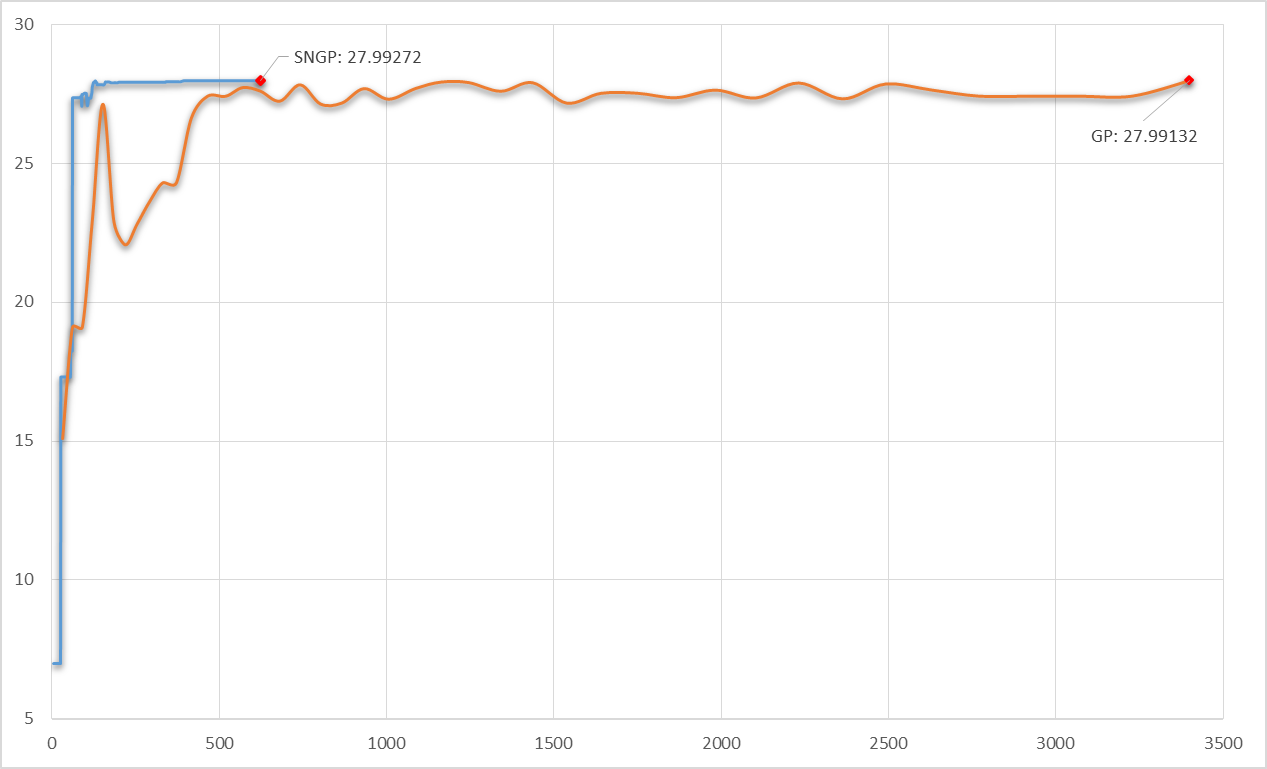
\includegraphics[keepaspectratio=true, width=300pt]{gpvssngp.png}
\end{frame}


\subsection{Sample SNGP vs GP Scalar Entropies}
\begin{frame}
\frametitle{Sample GP Scalar Entropies}
\begin{figure}[H]
\label{examplegraph}
\resizebox{300pt}{!}{
\begin{tikzpicture}
\begin{axis}[width=\textwidth, line width=0.7pt, font=\tiny, cycle list name=androidstyle, grid=major,grid style={dashed},
    xlabel={Time (Seconds)},
    ylabel={Entropy/Fitness (Bits)},
legend style={
at={(-0.055,0.34)},
anchor=north east}]
\addplot table [x=a, y=b, col sep=space, mark=none, smooth] {data5.dat};
\addplot table [x=a, y=c, col sep=space, mark=none, smooth] {data5.dat};
\addplot table [x=a, y=d, col sep=space, mark=none, smooth] {data5.dat};
\addplot table [x=a, y=e, col sep=space, mark=none, smooth] {data5.dat};
\addplot table [x=a, y=f, col sep=space, mark=none, smooth] {data5.dat};
\addplot table [x=a, y=g, col sep=space, mark=none, smooth] {data5.dat};
\addplot table [x=a, y=h, col sep=space, mark=none, smooth] {data5.dat};
\legend{1 Bit,2 Bit, 3 Bit, 4 Bit, 5 Bit, 6 Bit, 7 Bit}
%\addplot table [x=c, y=d, col sep=space, mark=none, smooth] {data.dat} node[pos=1,pin={[pin distance=2cm]265:{\textcolor{red}{GP} 3399.6 Sec 27.99132 Bits}}, inner sep=0pt] {};
%\addplot [color=blue, mark=x] coordinates {(624.599976, 27.99272)};
%\addplot [color=red, mark=x] coordinates {(3399.604004,27.99132)};
%\addplot [dash pattern=on 1pt off 3pt] table [x = e, y = f,  col sep=space] {data.dat};

%\addplot [dash pattern=on 1pt off 3pt] table [x = g, y = h,  col sep=space] {data.dat};
\end{axis}
%\draw node [above] {};
%\draw node [label={[rectangle, draw=blue, thick, fill=blue!20, align=center, rounded corners, minimum height=2em, font=\tiny,label distance=3.3cm]40:Comparsion of two successful, \\closest to average runs (with respect to run time)\\ of both SNGP and GP implementations.}] {};
%\draw node [label={[label distance=7cm, font=\tiny]80:Fitness threshold = 27.99 Bits of Entropy}] {};
\end{tikzpicture}
}
\end{figure}
%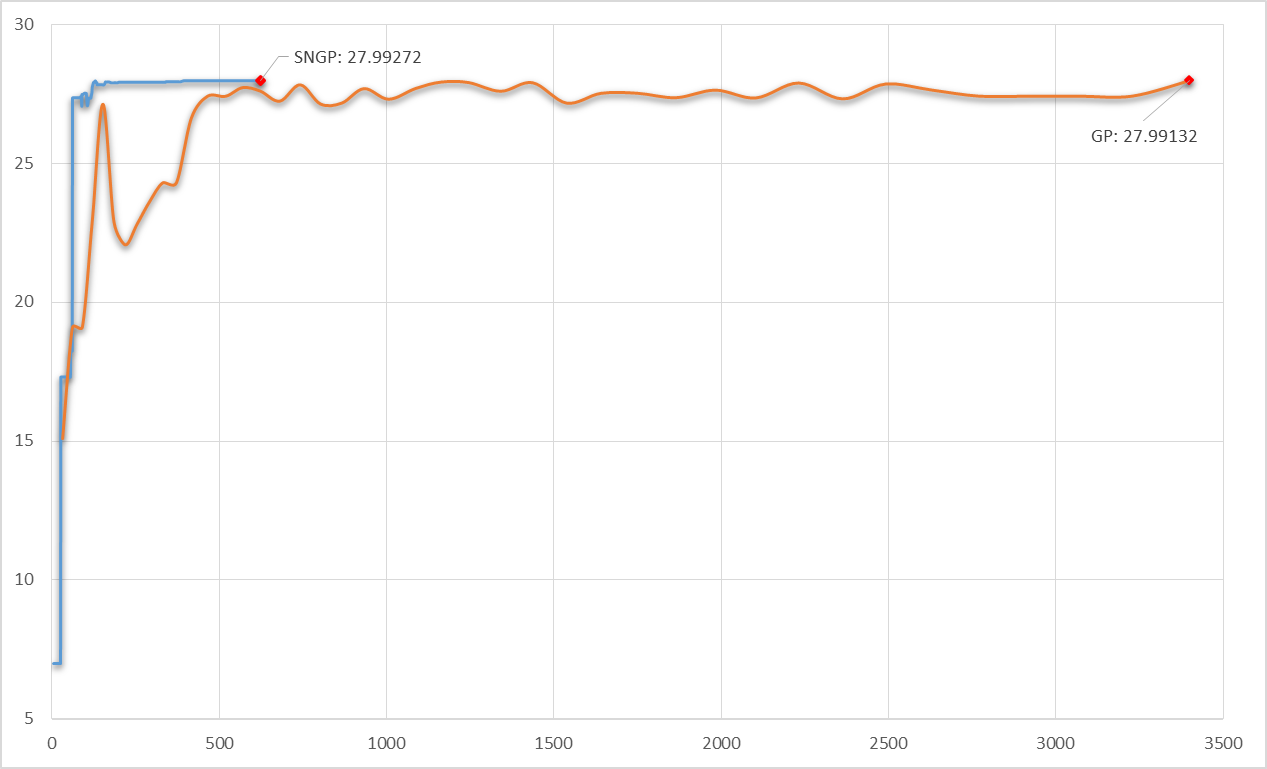
\includegraphics[keepaspectratio=true, width=300pt]{gpvssngp.png}
\end{frame}

\begin{frame}
\frametitle{Sample SNGP Scalar Entropies}
\begin{figure}[H]
\label{examplegraph}
\resizebox{300pt}{!}{
\begin{tikzpicture}
\begin{axis}[width=\textwidth, line width=0.7pt, font=\tiny,  cycle list name=androidstyle, grid=major,grid style={dashed},
    xlabel={Time (Seconds)},
    ylabel={Entropy/Fitness (Bits)},
legend style={
at={(-0.055,0.34)},
anchor=north east}]
\addplot table [x=a, y=b, col sep=space, mark=none, smooth, color=red] {data4.dat};
\addplot table [x=a, y=c, col sep=space, mark=none, smooth,  color=blue] {data4.dat};
\addplot table [x=a, y=d, col sep=space, mark=none, smooth,  color=green] {data4.dat};
\addplot table [x=a, y=e, col sep=space, mark=none, smooth,  color=red] {data4.dat};
\addplot table [x=a, y=f, col sep=space, mark=none, smooth] {data4.dat};
\addplot table [x=a, y=g, col sep=space, mark=none, smooth] {data4.dat};
\addplot table [x=a, y=h, col sep=space, mark=none, smooth] {data4.dat};
\legend{1 Bit,2 Bit, 3 Bit, 4 Bit, 5 Bit, 6 Bit, 7 Bit}
%\addplot table [x=c, y=d, col sep=space, mark=none, smooth] {data.dat} node[pos=1,pin={[pin distance=2cm]265:{\textcolor{red}{GP} 3399.6 Sec 27.99132 Bits}}, inner sep=0pt] {};
%\addplot [color=blue, mark=x] coordinates {(624.599976, 27.99272)};
%\addplot [color=red, mark=x] coordinates {(3399.604004,27.99132)};
%\addplot [dash pattern=on 1pt off 3pt] table [x = e, y = f,  col sep=space] {data.dat};

%\addplot [dash pattern=on 1pt off 3pt] table [x = g, y = h,  col sep=space] {data.dat};
\end{axis}
%\draw node [above] {};
%\draw node [label={[rectangle, draw=blue, thick, fill=blue!20, align=center, rounded corners, minimum height=2em, font=\tiny,label distance=3.3cm]40:Comparsion of two successful, \\closest to average runs (with respect to run time)\\ of both SNGP and GP implementations.}] {};
%\draw node [label={[label distance=7cm, font=\tiny]80:Fitness threshold = 27.99 Bits of Entropy}] {};
\end{tikzpicture}
}
\end{figure}
%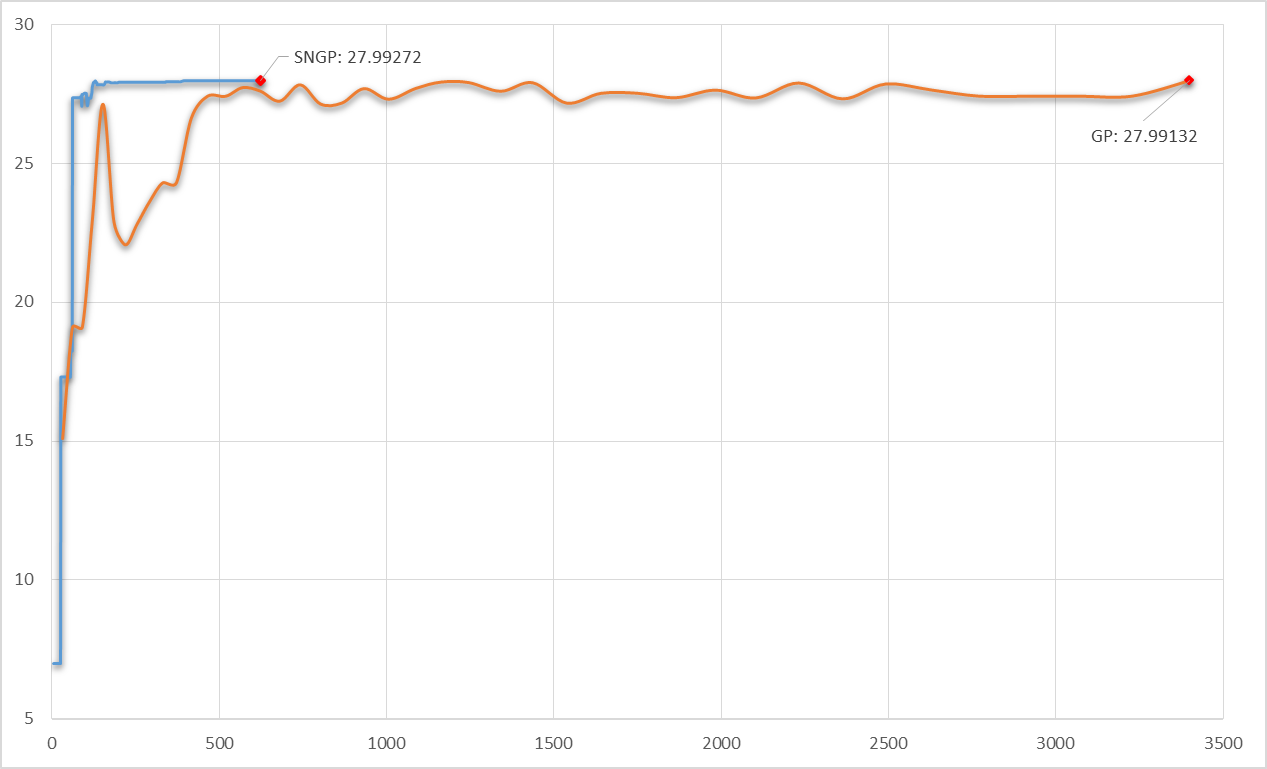
\includegraphics[keepaspectratio=true, width=300pt]{gpvssngp.png}
\end{frame}

\subsection{50 Run Average GP vs SNGP}
\begin{frame}
\frametitle{50 Run Average GP vs SNGP}
After 50 Runs of both implementations, I was able to gather some promising data. The results show that SNGP is both quicker and more effective than GP when it comes to finding solutions (I.e. RNGs with entropy higher than 27.99)

\begin{table}
    \begin{tabular}{l|l|l}
    ~                 & SNGP           & GP             \\ \hline
    Avg Run Time      &    \textcolor{red}{606.9s} &    4111.6s \\
    Avg Sol Run Time  & \textcolor{red}{483.2s}    & 2173.4s   \\
    Solution Rate     & \textcolor{red}{88\%}           & 40\%           \\
    Avg Sol Size      & 167.5  & \textcolor{red}{154.6}          \\
    Avg Final Size    & \textcolor{red}{167.3}        & 277.8          \\
    Avg Run Fitness   & \textcolor{red}{27.88153318}    &  27.2570626    \\
    Best Sol Fitness  & \textcolor{red}{27.995729}      & 27.995032      \\
    Avg Sol Fitness   & 27.9917378     & \textcolor{red}{27.99195145}    \\
    \end{tabular}
\end{table}

\end{frame}

\subsection{50 Run C Rand() vs Random.org vs GP vs SNGP}
\begin{frame}
\frametitle{50 Run C Rand() vs Random.org vs GP vs SNGP}
I also collected data from 50 calls of both the C Rand function (seeded with the time), and atmospheric noise data from Random.org. The results are promising, showing that the RNGs produced genetically fractionally outperform both common methods of producing random numbers.
\begin{table}
\resizebox{11cm}{!}{
    \begin{tabular}{l|l|l|l|l}
    ~                     & TRNG           & C PRNG         & SNGP           & GP             \\ \hline
    Fittest (Entropy)               &    27.993097   &    27.991925   &    \textcolor{red}{27.995729}   &    27.995032   \\ \hline
    Fittest (\%)               &    99.975\%  &    99.9712\%  &    \textcolor{red}{99.985\%}   &    99.982\%  \\ \hline
    Fittest (Entropy Shortfall)               &    0.006903   &    0.008075  &    \textcolor{red}{0.004271}   &    0.004968   \\ \hline
    Avg Fit (Entropy) (Sol) &    27.98695522 &    27.98985372 &    27.9917378  &    \textcolor{red}{27.99195145} \\ \hline
   Avg Fit (\%) (Sol) &    99.953\% &    99.964\% &   99.970\%  &    \textcolor{red}{99.971\%} \\ \hline
   Avg Fit (Shortfall) (Sol) &    0.01304478 &   0.01014628 &    0.0082622  &    \textcolor{red}{0.00804855} \\ 
    \end{tabular}}
\end{table}
\end{frame}

\subsection{Graphical Data}
\begin{frame}
\frametitle{Random.org Entropy Fluctuation Over Time}
The entropy fluctuation on the day which I gathered the data from Random.org is shown on the graph below generated by their servers.
\begin{center}
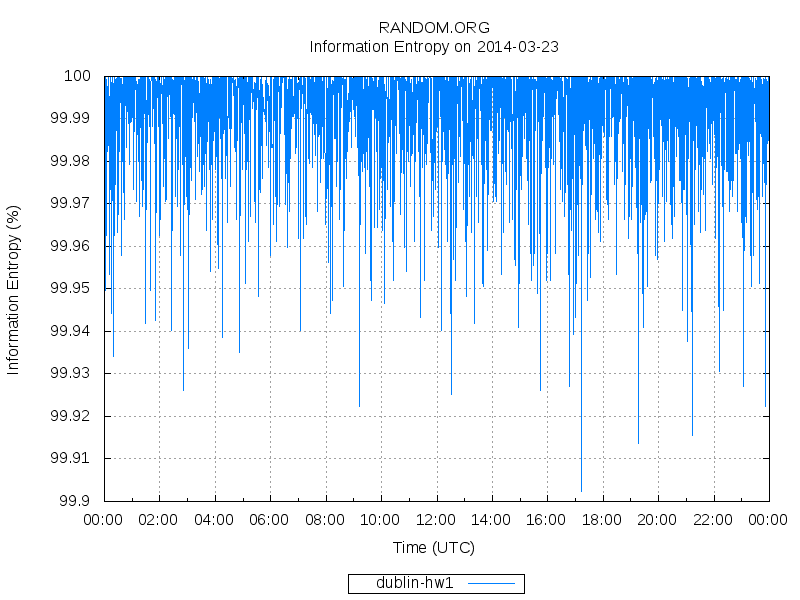
\includegraphics[keepaspectratio=true, height= 200pt]{2014-03-24.png}
\end{center}
\end{frame}




\begin{frame}
\frametitle{SNGP Entropy Shortfall of Solutions}
\begin{figure}[H]
\label{examplegraph}
\resizebox{300pt}{!}{
\begin{tikzpicture}
\begin{axis}[x=8pt, width=\textwidth, line width=0pt, font=\tiny, bar width=3pt, axis on top, ymax=100, ymin=99.93, grid=major,grid style={dashed}, xmin = 0.5, xmax = 45.5,  line width=0.7pt, smooth,
stack plots=y,
area style,
enlarge x limits=false,
    xlabel={Run Number},
    ylabel={Entropy (\%)}]]

\addplot [lblue] table [x= a, y=c] {data2.dat};    % Plot the "First" column against the data index
%\addplot [lblue, fill=lblue, mark=none]table [x = a, y=d] {data2.dat};

\end{axis}
%\draw node [above] {};
%\draw node [label={[rectangle, draw=blue, thick, fill=blue!20, align=center, rounded corners, minimum height=2em, font=\tiny,label distance=3.3cm]40:Comparsion of two successful, \\closest to average runs (with respect to run time)\\ of both SNGP and GP implementations.}] {};
%\draw node [label={[label distance=13.8cm, rotate=-90]93:Max Gen \# or $smut$ operations = 51}] {};
\draw node [label={[rectangle, draw=blue, thick, fill=blue!20, align=center, rounded corners, minimum height=2em, font=\tiny,label distance=3.2cm]10:Entropy shortfall from 28 bits for all \\the solutions produced by the SNGP implementation}] {};
\end{tikzpicture}
}
\end{figure}
\end{frame}

\begin{frame}
\frametitle{GP Entropy Shortfall of Solutions}
\begin{figure}[H]
\label{examplegraph}
\resizebox{300pt}{!}{
\begin{tikzpicture}
\begin{axis}[x=18pt, width=\textwidth, line width=0pt, font=\tiny, bar width=8pt, axis on top, ymin=99.93, grid=major, grid style={dashed}, xmin = 0.5, xmax =20.5,ymax=100, line width=0.7pt, smooth,
stack plots=y,
area style,
enlarge x limits=false,
    xlabel={Run Number},
    ylabel={Entropy (\%)}]]

\addplot [lred] table [x= a, y=b] {data3.dat};    % Plot the "First" column against the data index
%\addplot [fill=lred, lred]table [x = a, y=c] {data3.dat};

\end{axis}
%\draw node [above] {};
%\draw node [label={[rectangle, draw=blue, thick, fill=blue!20, align=center, rounded corners, minimum height=2em, font=\tiny,label distance=3.3cm]40:Comparsion of two successful, \\closest to average runs (with respect to run time)\\ of both SNGP and GP implementations.}] {};
%\draw node [label={[label distance=13.8cm, rotate=-90]93:Max Gen \# or $smut$ operations = 51}] {};
\draw node [label={[rectangle, draw=blue, thick, fill=blue!20, align=center, rounded corners, minimum height=2em, font=\tiny,label distance=4.7cm]8:Entropy shortfall from 28 bits for all \\the solutions produced by the GP implementation}] {};
\end{tikzpicture}
}
\end{figure}
\end{frame}

\begin{frame}
\frametitle{SNGP Surface Plot}
A graphical view of the correlation between running time, solution size and Entropy of all 50 runs of the Single Node Genetic Programming Implementation.
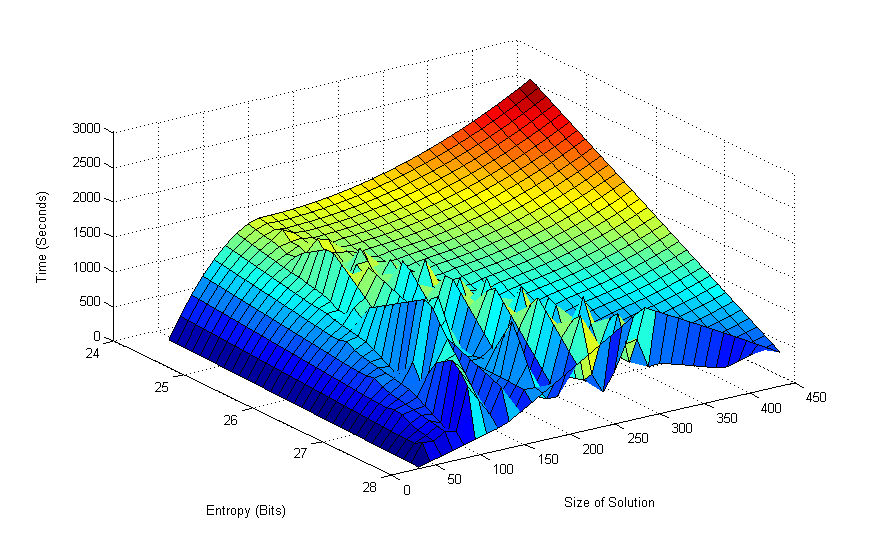
\includegraphics[keepaspectratio=true, height= 200pt]{sngp.png}
\end{frame}

\begin{frame}
\frametitle{Genetic Programming Surface Plot}
A graphical view of the correlation between running time, solution size and Entropy of all 50 runs of the Genetic Programming Implementation.
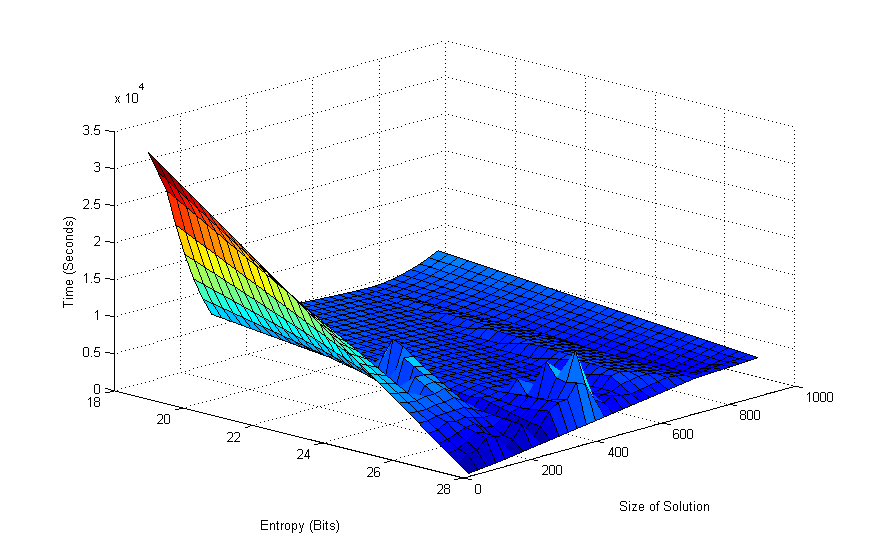
\includegraphics[keepaspectratio=true, height= 200pt]{gp.png}
\end{frame}

\begin{frame}
\frametitle{Overview}
To conclude, it is clearly evident that SNGP produces more solutions in a much quicker time frame, under these standard parameters. It is also evident that a RNG produced genetically can outperform common pseudo and natural methods of producing random numbers.\newline

This has just been a snapshot of the evaluation, in my dissertation further analysing of both GP and SNGP will be undertaken using different parameters in order to observe performance under different conditions.

\end{frame}


\section{Progress}
\begin{frame}
\frametitle{Progress}
\begin{figure}

\resizebox{11.5cm}{6cm}{
\centering
\begin{ganttchart}[y unit title=0.4cm,
y unit chart=0.5cm,
vgrid,hgrid, 
title label anchor/.style={below=-1.6ex},
title height=1,
bar/.style={fill=gray!50},
bar/.append style={fill=gray!100},
bar incomplete/.append style={fill=gray!50},
incomplete/.style={fill=white},
progress = today,
today = 28, 
bar height=0.7,
group right shift=0,
group top shift=.6,
group height=.3,
group peaks height =.2,
milestone/.append style={fill=gray!50}
]
{1}{34}
%labels
\gantttitle{Final Year Project}{34} \\
\gantttitle{Sep}{2} 
\gantttitle{Oct}{4} 
\gantttitle{Nov}{4} 
\gantttitle{Dec}{4} 
\gantttitle{Jan}{4} 
\gantttitle{Feb}{4} 
\gantttitle{Mar}{4} 
\gantttitle{Apr}{4} 
\gantttitle{May}{4} \\
%tasks
\ganttbar{Research}{1}{6} \\
\ganttgroup{Specification}{2}{4} \\
\ganttbar{Write Specification}{2}{4} \\
\ganttgroup{Design}{5}{10} \\
\ganttbar{Plan Design}{5}{5}\\
\ganttbar{Write Design Document}{6}{9}\\
\ganttbar{Plan Presentation}{9}{9}\\
\ganttbar{Give Design Presentation}{10}{10} \\
\ganttmilestone{Implementation Documentation Complete}{10}\\
\ganttgroup{Implementation}{11}{26} \\
\ganttbar{Implement Koza's PRNG GP}{11}{18}\\
\ganttbar{Implement SNGP Approach}{19}{23} \\
\ganttbar{Compare GP vs SNGP}{24}{26}\\
\ganttmilestone{Implementation Complete}{26} \\
\ganttgroup{Demonstration}{27}{28} \\
\ganttbar{Write/Plan Demonstration}{27}{27} \\
\ganttbar{Give Demonstration}{28}{28} \\
\ganttgroup{Dissertation}{29}{34} \\
\ganttbar{Plan Dissertation}{29}{29}\\
\ganttbar{Write Dissertation}{30}{34} \\
\ganttmilestone{Project Completed}{34} \\

%relations
\ganttlink[link type=dr]{elem2}{elem4} 
\ganttlink[link type=dr]{elem4}{elem5}
\ganttlink[link type=dr]{elem4}{elem6}
\ganttlink[link type=dr]{elem5}{elem8}
\ganttlink[link type=dr]{elem6}{elem7}
\ganttlink[link type=dr]{elem7}{elem8} 
\ganttlink[link type=dr]{elem8}{elem10} 
\ganttlink[link type=dr]{elem10}{elem11}
\ganttlink[link type=dr]{elem10}{elem12}
\ganttlink[link type=dr]{elem11}{elem12}
\ganttlink[link type=dr]{elem12}{elem13} 
\ganttlink[link type=dr]{elem13}{elem15}
\ganttlink[link type=dr]{elem15}{elem16}
\ganttlink[link type=dr]{elem16}{elem18}
\ganttlink[link type=dr]{elem18}{elem19}
\ganttlink[link type=dr]{elem19}{elem20}

\end{ganttchart}}
\caption{Gantt Chart - Work plan}
\label{fig:ganttchart}
\end{figure}

\end{frame}

\begin{thebibliography}{2}
\bibitem{kozarng}
  John R. Koza, 
  \emph{Evolving a Computer Program to Generate Random Numbers Using the Genetic Programming Paradigm}. 
  Stanford University, 
  1991.

\bibitem{jacksonsngp2}
  David Jackson,
  \emph{A New, Node-Focused Model for Genetic Programming}.
  Proceedings of the 15th European Conference on Genetic Programming, EuroGP 2012, 
  Springer Verlag
  2012.
\end{thebibliography}

\begin{frame}
\begin{center}Q\&A\end{center}
\end{frame}
\end{document} 